\documentclass[a4paper, 12pt]{article}

% a nice font
\usepackage{kpfonts}

% basic text stuff
\usepackage[utf8]{inputenc}
\usepackage[T1]{fontenc}

\usepackage{colortbl} % to color rows or columns of matrices

\usepackage{tikz} % main tikz package
\usepackage{tikz-network} % provides graph / network utilities (Edge, Node, etc)

\usetikzlibrary{calc} % to do some computations on the coordinates

% for a nicer colorscheme
\definecolor{blue}{rgb}{0.38, 0.51, 0.71} %glaucous, 97,130,181, #6182B5
\definecolor{darkblue}{RGB}{17, 42, 60} % 112A3C
\definecolor{red}{RGB}{175, 49, 39} % AF3127

\definecolor{orange}{RGB}{217, 156, 55} % D99C37
\definecolor{green}{RGB}{144, 169, 84} % 90A954
\definecolor{palegreen}{RGB}{197, 184, 104} % C5B868

\definecolor{yellow}{RGB}{250, 199, 100} % FAC764
\definecolor{brokenwhite}{RGB}{218, 192, 166} % DAC0A6
\definecolor{brokengrey}{rgb}{0.77, 0.76, 0.82} % {196,194,209}, C4C2D1


\begin{document}
    \begin{tikzpicture}[>=stealth']
        \node (g1) at (0,0) {\begin{tikzpicture}[scale=0.3, every node/.style={scale=0.7}]
                                \Vertex[x=3.9,y=2.1,size=0.3,color={196,193,209},RGB]{0}
                                \Vertex[x=4.6,y=3.8,size=0.3,color={196,193,209},RGB]{1}
                                \Vertex[x=3.3,y=3.4,size=0.3,color={196,193,209},RGB]{2}
                                \Vertex[x=2.5,y=4.4,size=0.3,color={196,193,209},RGB]{3}
                                \Vertex[x=2.7,y=5.6,size=0.3,color={196,193,209},RGB]{4}
                                \Vertex[x=1.4,y=5.5,size=0.3,color={196,193,209},RGB]{5}
                                \Vertex[x=0.5,y=4.7,size=0.3,color={196,193,209},RGB]{6}
                                \Vertex[x=1.8,y=3.2,size=0.3,color={196,193,209},RGB]{7}
                                \Vertex[x=0.2,y=3.1,size=0.3,color={196,193,209},RGB]{8}
                                \Vertex[x=0.8,y=1.6,size=0.3,color={196,193,209},RGB]{9}
                                \Vertex[x=0.5,y=0.7,size=0.3,color={196,193,209},RGB]{10}
                                \Vertex[x=2.5,y=0.3,size=0.3,color={196,193,209},RGB]{11}
                                \Vertex[x=2.2,y=1.4,size=0.3,color={196,193,209},RGB]{12}
                                \Vertex[x=5.6,y=1.0,size=0.3,color={196,193,209},RGB]{13}
                                \Vertex[x=5.8,y=2.6,size=0.3,color={196,193,209},RGB]{14}
                                \Edge[,bend=-8.5](0)(1)
                                \Edge[,bend=-8.5](0)(14)
                                \Edge[,bend=-8.5](0)(2)
                                \Edge[,bend=-8.5](0)(13)
                                \Edge[,bend=-8.5](0)(7)
                                \Edge[,bend=-8.5](0)(11)
                                \Edge[,bend=-8.5](1)(2)
                                \Edge[,bend=-8.5](1)(3)
                                \Edge[,bend=-8.5](1)(14)
                                \Edge[,bend=-8.5](2)(3)
                                \Edge[,bend=-8.5](2)(4)
                                \Edge[,bend=-8.5](2)(12)
                                \Edge[,bend=-8.5](3)(4)
                                \Edge[,bend=-8.5](3)(5)
                                \Edge[,bend=-8.5](3)(8)
                                \Edge[,bend=-8.5](4)(5)
                                \Edge[,bend=-8.5](4)(6)
                                \Edge[,bend=-8.5](5)(6)
                                \Edge[,bend=-8.5](5)(7)
                                \Edge[,bend=-8.5](6)(7)
                                \Edge[,bend=-8.5](6)(8)
                                \Edge[,bend=-8.5](7)(9)
                                \Edge[,bend=-8.5](8)(10)
                                \Edge[,bend=-8.5](9)(10)
                                \Edge[,bend=-8.5](9)(11)
                                \Edge[,bend=-8.5](9)(12)
                                \Edge[,bend=-8.5](10)(11)
                                \Edge[,bend=-8.5](10)(12)
                                \Edge[,bend=-8.5](11)(12)
                                \Edge[,bend=-8.5](13)(14)
                             \end{tikzpicture}};
        \node (g2) at (7,0) {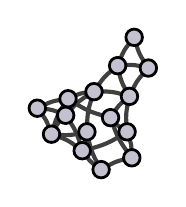
\begin{tikzpicture}[scale=0.3, every node/.style={scale=0.7}]

                                    \Vertex[x=2.5,y=1.0,size=0.3,color={196,193,209},RGB]{0}
                                    \Vertex[x=4.7,y=5.8,size=0.3,color={196,193,209},RGB]{1}
                                    \Vertex[x=5.3,y=4.5,size=0.3,color={196,193,209},RGB]{2}
                                    \Vertex[x=4.0,y=4.6,size=0.3,color={196,193,209},RGB]{3}
                                    \Vertex[x=4.5,y=3.3,size=0.3,color={196,193,209},RGB]{4}
                                    \Vertex[x=3.0,y=3.5,size=0.3,color={196,193,209},RGB]{5}
                                    \Vertex[x=1.8,y=2.5,size=0.3,color={196,193,209},RGB]{6}
                                    \Vertex[x=1.9,y=3.2,size=0.3,color={196,193,209},RGB]{7}
                                    \Vertex[x=1.2,y=1.7,size=0.3,color={196,193,209},RGB]{8}
                                    \Vertex[x=2.7,y=1.8,size=0.3,color={196,193,209},RGB]{9}
                                    \Vertex[x=0.6,y=2.8,size=0.3,color={196,193,209},RGB]{10}
                                    \Vertex[x=3.7,y=2.4,size=0.3,color={196,193,209},RGB]{11}
                                    \Vertex[x=4.6,y=0.7,size=0.3,color={196,193,209},RGB]{12}
                                    \Vertex[x=4.4,y=1.8,size=0.3,color={196,193,209},RGB]{13}
                                    \Vertex[x=3.3,y=0.2,size=0.3,color={196,193,209},RGB]{14}
                                    \Edge[,bend=-8.5](0)(14)
                                    \Edge[,bend=-8.5](0)(13)
                                    \Edge[,bend=-8.5](0)(8)
                                    \Edge[,bend=-8.5](0)(6)
                                    \Edge[,bend=-8.5](0)(9)
                                    \Edge[,bend=-8.5](1)(2)
                                    \Edge[,bend=-8.5](1)(3)
                                    \Edge[,bend=-8.5](2)(3)
                                    \Edge[,bend=-8.5](2)(4)
                                    \Edge[,bend=-8.5](3)(4)
                                    \Edge[,bend=-8.5](3)(5)
                                    \Edge[,bend=-8.5](4)(5)
                                    \Edge[,bend=-8.5](4)(13)
                                    \Edge[,bend=-8.5](4)(11)
                                    \Edge[,bend=-8.5](5)(6)
                                    \Edge[,bend=-8.5](5)(7)
                                    \Edge[,bend=-8.5](5)(9)
                                    \Edge[,bend=-8.5](6)(7)
                                    \Edge[,bend=-8.5](6)(8)
                                    \Edge[,bend=-8.5](6)(10)
                                    \Edge[,bend=-8.5](7)(8)
                                    \Edge[,bend=-8.5](7)(10)
                                    \Edge[,bend=-8.5](7)(11)
                                    \Edge[,bend=-8.5](8)(9)
                                    \Edge[,bend=-8.5](8)(10)
                                    \Edge[,bend=-8.5](9)(14)
                                    \Edge[,bend=-8.5](11)(12)
                                    \Edge[,bend=-8.5](11)(13)
                                    \Edge[,bend=-8.5](12)(13)
                                    \Edge[,bend=-8.5](12)(14)
                              \end{tikzpicture}};
        \node (n1) at (1,2) {$\mathcal{N}(0, L_1^{-1})$};
        \node (n2) at (6,2) {$\mathcal{N}(0, L_2^{-1})$};
        \draw[<->, thick, bend right = -5, bend left=-5] (g1) to node [below] {graph distance?} (g2);
        \draw[->, dashed, bend left = 30] (g1) to (n1.west);
        \draw[->, dashed, bend right = 30] (g2) to (n2.east);
        \draw[<->, thick, bend right = 5, bend left=5] (n1) to node [above] {optimal transport} (n2);
    \end{tikzpicture}

\end{document}
